\documentclass[10pt]{article}

\usepackage{amsmath}
\usepackage{amssymb}
\usepackage{graphicx}

\counterwithin*{equation}{section}
\counterwithin*{equation}{subsection}
\addtolength\parskip{\bigskipamount}

\graphicspath{ {./images/} } 

\begin{document}
\section{Vectors}
Vectors have a magnitude(length) and direction.\\
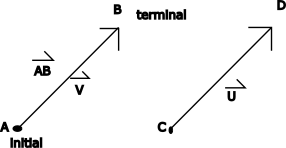
\includegraphics{somevectors}\\ $\vec{u}$ \& $\vec{v}$ have the same direction and magnitude, $\therefore$ they are equivalent.

\underline{Zero Vector} $\vec{O}$ has length zero. 

Vectors appear in forces, position, velocity, acceleration, torque, displacement, images.

\underline{Sums} $\vec{u}+\vec{v} = \vec{v}+\vec{u}$ 
 
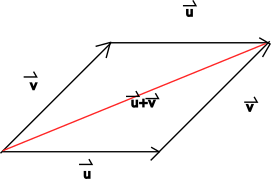
\includegraphics{sumvector} 
 
\underline{Scalar Multiplication}
\begin{itemize}
	\item If $c\in\mathbb{R}$, then vector $c \vec{v}$ has length |c| times the length of $\vec{v}$ and \begin{itemize} 
		\item the same direction as $\vec{v}$ if $c > 0$ 
		\item opposite direction as $\vec{v}$ if $c < 0$ 
	\end{itemize}
	\item If $c=0$ or $\vec{v} = \vec{o}$, then $c \vec{v} = 0$ 
\end{itemize}

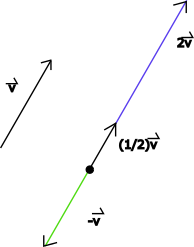
\includegraphics{scalarmult}

\underline{Differences} $\vec{u} - \vec{v} = \vec{u} + (-\vec{v})$ 

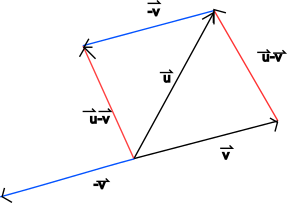
\includegraphics{vectordifference}

\underline{Ex:} Consider $\vec{u}\ and\ \vec{v}   $. Sketch $2 \vec{u}-\vec{v}$  

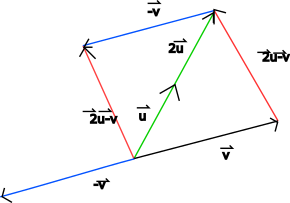
\includegraphics{vectordifference2}

\underline{Components}

\underline{2D:} $\vec{a} = <,a,b> $

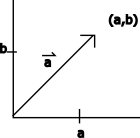
\includegraphics{vectorcomponents2d}

\underline{3D:} $\vec{a}=<a,b,c>  $

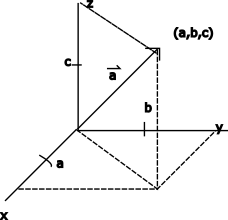
\includegraphics{vectorcomponents3d}

Sketch vectors equivalent to $\vec{a} = <2, -1>$ \\Choose any initial position in the graph. So long as it obeys the magnitude and direction of the vector it is valid.

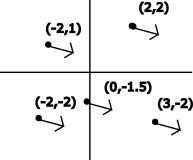
\includegraphics{equivalentvectors2d}

Unmarked in the graph is the point $o \vec{P}  $ which is the position vector for point $P$, otherwise known as the \underline{origin}.

Find components of the vector $\vec{a}  $ that has the following:\\\underline{Initial Point}: $(3,1)$\\\underline{Terminal Point}: $(-2,5)$

Vector $\vec{a}  $ has point $(-2-3,5-1)=(-5,4)$

Find components of the vector $\vec{b}  $ that has the following:\\\underline{Initial Point}: $(1,2,3)$\\\underline{Terminal Point}: $(-2,5,-7)$

Vector $\vec{a}  $ has point $(-2-1,5-2,-7-3)=(-3,3,-10)$

To sum up,
In general $\vec{AB}  $ has components $B(x_2,y_2),\ A(x_1,y_1) $ and is the result of $\vec{AB} =<x_2-x_1,y_2-y_1> $

Vector $\vec{ABC}  $ has components $B(x_2,y_2,z_2),\ A(x_1,y_1,z_1)$.\\It is the result of $\vec{ABC} =<x_2-x_1,y_2-y_1,z_2-z_1> $ 

Practice:

\underline{EX:} Let $\vec{a} =<0,4,3>\ and\ \vec{b} =<1,-2,5>.  $ Find:

\begin{enumerate}
	\item $|\vec{a} |\ = \sqrt{0^2+4^2+3^2}=\sqrt{25}=5 $
	\item $\vec{a} +\vec{b}\ =<0,4,3>+<1,-2,5>\\=<0+1,4+(-2),3+5>\\=<1,2,8>  $
	\item $\vec{a} -\vec{b}\ =<0-1,4-(-2),3-5>=<-1,6,-2> $
	\item $4\vec{b}\  =<4(1),4(-2),4(5)>\\=<4,-8,20>$ 
	\item $3 \vec{a} +2 \vec{b}\ = 3<0,4,3>+2<1,-2,5>\\=<0+2,12+(-4),9+10>\\=<2,8,19>  $
\end{enumerate}

\underline{Notation}
\begin{itemize}
	\item $V_2=$\{all 2D vectors\}$=\mathbb{R}^2=\{<a,b>:a,b\in\mathbb{R}\}$
	\item $V_3=$\{all 3D vectors\}$=\mathbb{R}^3$
	\item $V_n=$\{all n-dimensional vectors\}$=\mathbb{R}^n$
	\item $\mathbb{R}^\infty=\{(a_1,a_2,a_3,\hdots):a_i\in\mathbb{R}\}$
\end{itemize}

\underline{Ideas:} If $\vec{a} \in V_n $ then $\vec{a}  = <a_1,a_2,\hdots,a_n> $

\underline{Properties}

If $\vec{a} , \vec{b} , \vec{c} \in V_n\ and\ c\&d   $ are scalars, then:
\begin{itemize}
	\item $\vec{a} + \vec{b}  = \vec{b}  + \vec{a}     $: commutative property
	\item $\vec{a} +(\vec{b} +\vec{c} )=(\vec{a} +\vec{b} )+\vec{c}       $: associative property
	\item $\vec{a} +\vec{0} =\vec{a}    $: additive identity
	\item $\vec{a} +(\vec{-a} )=\vec{0}    $: additive inverse 
	\item $c(\vec{a} +\vec{b} )=c \vec{a} + c \vec{b}     $: distributive property
	\item $(c+d)\vec{a} =c \vec{a}  + d \vec{a}    $: distributive property
	\item $(cd>\vec{a} =c(d \vec{a} )  $: associative property
	\item $1 \vec{a} =\vec{a}   $
\end{itemize}

\underline{Standard Basis Vectors}\\Set of vectors whose components are all zero except one which equals 1.

In 2D:\\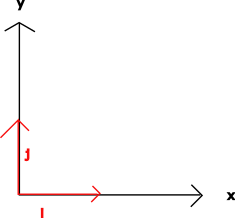
\includegraphics{standardbasisvectors} $\hat{i}=<1,0>,\ \hat{j}=<0,1>$

The following equation describes the components of a vector $\vec{a}  $ using standard basis vectors.

$\vec{a} =<a_1,a_2>\\=a_1<1,0>+a_2<0,1>\\=a_1\hat{i}+a_2\hat{j} $

In 3D:\\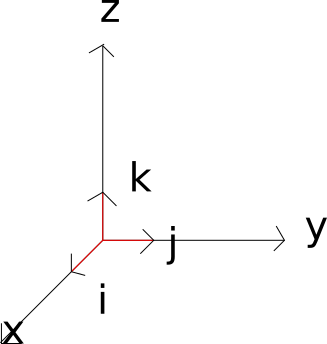
\includegraphics{3dstandardbasisvectors} 

The following equation describes the components of a vector $\vec{a}$ using standard basis vectors.
\begin{align}
	\vec{a} =<a_1,a_2,a_3>\\ =a_1<1,0,0>+a_2<0,1,0>+a_3<0,0,1>\\	=a_1\hat{i}+a_2\hat{j}+a_3\hat{k}  
\end{align}

\end{document}
